Now we apply the properties discussed in the last chapter onto connected graphs to demonstrate their use. These properties are used to outline and modify the graph such that an alternative layout may be given. A different layout means a new visualisation that can reveal correlations between the vertices or edges. By using Python, I have coded a program to display a graph either generated from an adjacency matrix, a weighted matrix or a dataset that is pre-existing. To help accomplish this, I have used Tiago P. Peixoto's Graph Tool library for python \cite{peixoto_graph-tool_2014} which contains useful documentation and functions to achieve the graph generations. Along with Peixoto's library, I have used other mathematical libraries for complex arithmetic. The general idea is to compare various graph properties by modifying their positions according to the values of their graph properties. For simplicity and the goal of being comparable, we choose the $y$-axis of the graph to be based upon the trophic levels and the $x$-axis to vary between the different properties discussed in the last chapter.

\section{Early Experimentations}
Out of the many pre-existing datasets from the graph tool library, I chose to experiment on a smaller dataset that demonstrates the relationships between karate clubs in a city. This is so that I can test and generate a visualisation of this dataset before beginning the linguistic analysis. This dataset involves 34 karate clubs and the initial graph can be seen by Figure \ref{fig:karate}. This is also to test that the visualisations are viable for a simple undirected graph prior to directed graphs. However, the trophic levels are not used ideally in this scenario as they focus on directed graphs and their hierarchical structure. Consequently, they will be analysed thoroughly in linguistic analysis later and will not be analysed for this karate dataset.

\begin{figure}[!htb]
	\centering
	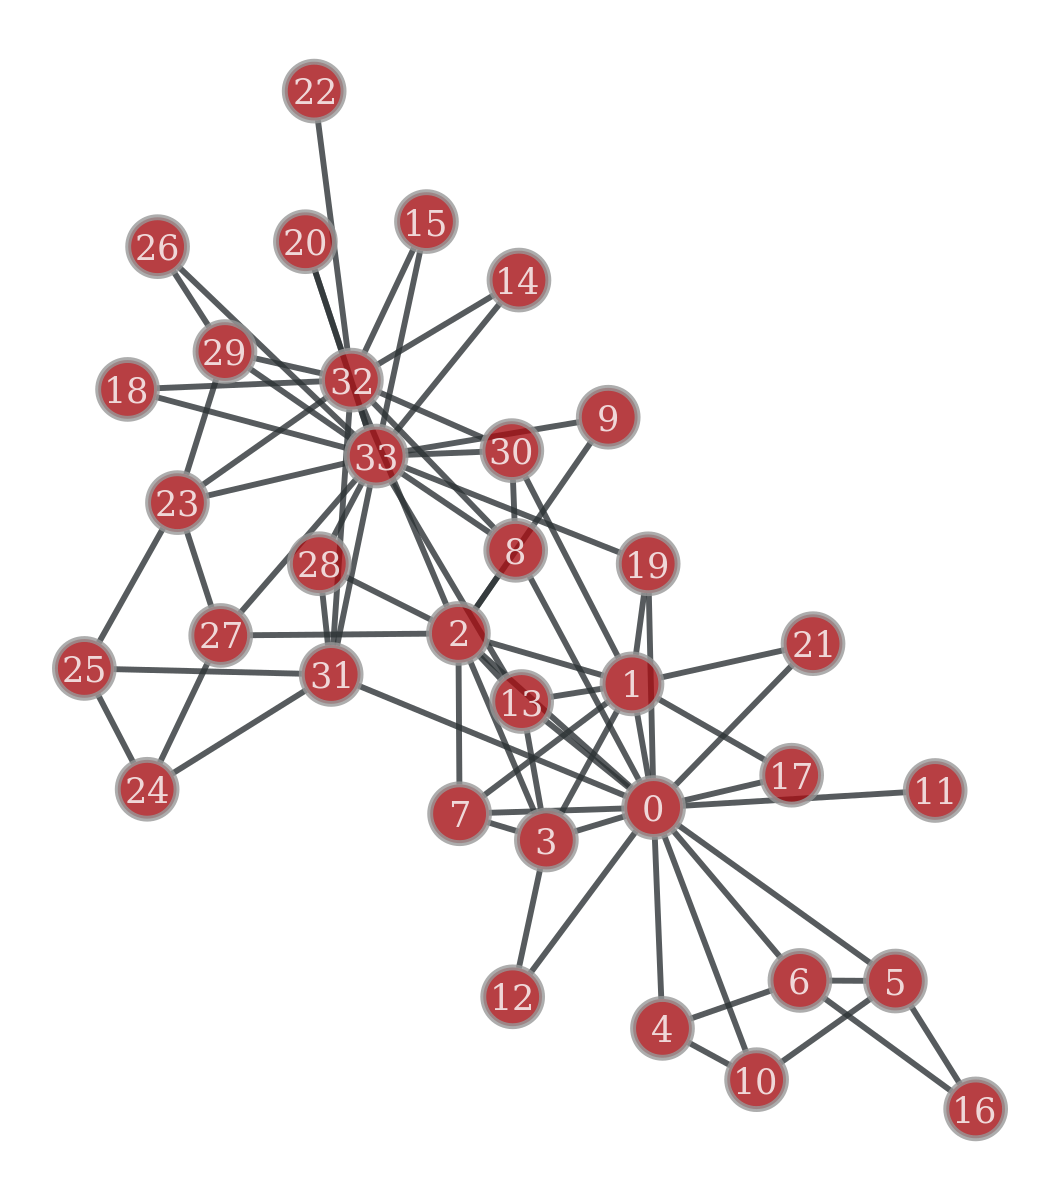
\includegraphics[scale=0.25]{karate.png}
	\caption{The initial graph based on the karate club dataset pre-existing within the library that was generated through the python program. Contains 34 clubs and their connections to one another with no important meaning with the positions of the vertices.}
	\label{fig:karate}
\end{figure}

The current positioning of the graph is determined based on the idea that the vertices do not overlap with each other, and their connections are easily visible. So, the positioning of the elements in the dataset has no real benefits other than having good visibility. Any correlations or vital information cannot be derived from the initial graph. The only information that can be derived by initial examination are the certain outliers who only have one edge, vertices 22 and 11. Thus, we now include various graph properties discussed in the last chapter to ensure that more can be visualised. This can be seen in Figures \ref{fig:karatecentrality} and \ref{fig:karatelocal} by using the trophic levels values for each vertex as their $y$-value and another property value for their $x$-value.

For karate clubs, the trophic levels do not represent a clear hierarchical format due to the undirected edges as there is no distinction between ``upstream" or ``downstream" of information. Even though they may not be accurate, we use them temporarily to distinguish the vertices as they can implement some structure into the karate dataset. Further datasets involving languages will be directional so that trophic levels can be used optimally.

\begin{figure}[!htb]
\centering
\begin{subfigure}{.45\textwidth}
	\hspace{-2cm}
	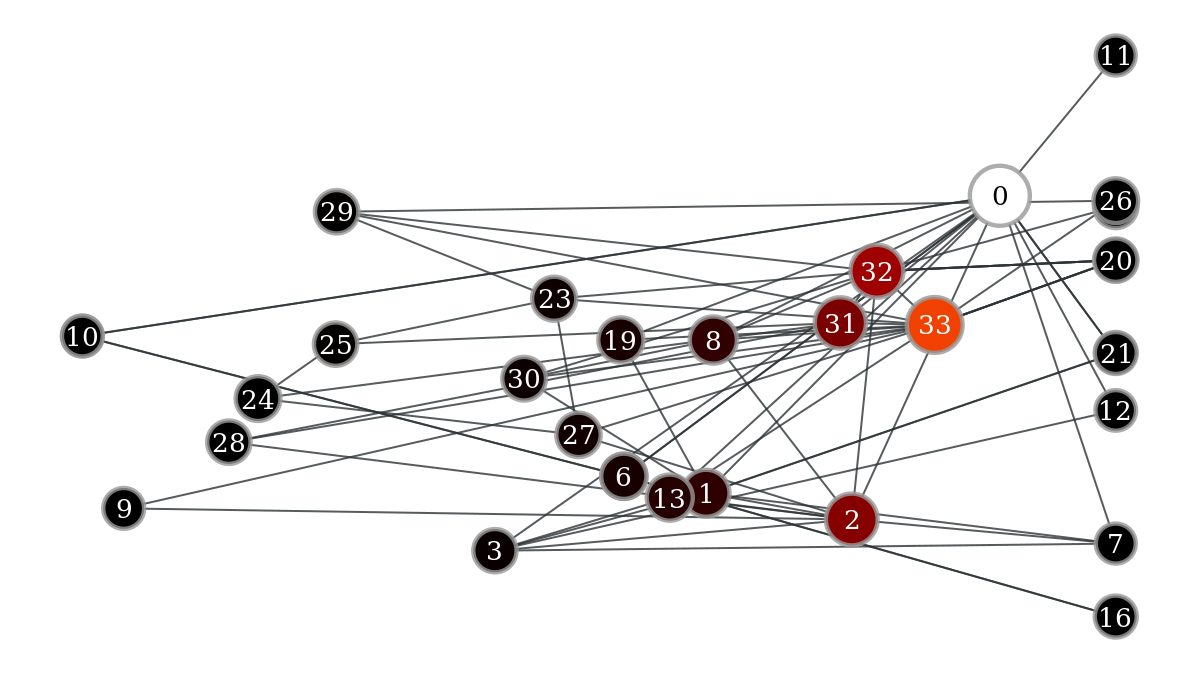
\includegraphics[scale=0.7]{karatebetween.png}
	\caption{}
	\label{fig:karatea}
\end{subfigure}
\begin{subfigure}{.45\textwidth}
	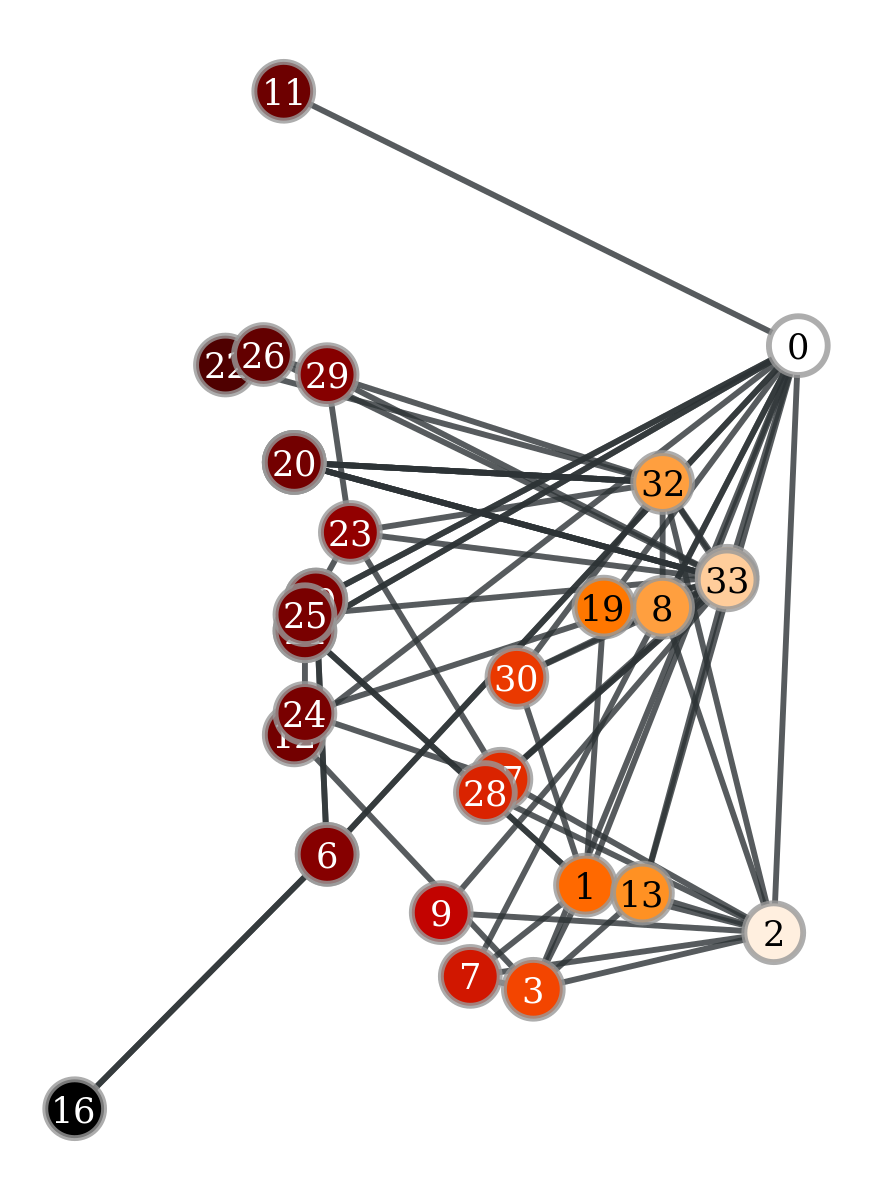
\includegraphics[scale=0.7]{karatecloseness.png}
	\caption{}
	\label{fig:karateb}
\end{subfigure}
\caption{Graph generated by karate dataset, the $y$-axis represents the trophic levels, and the $x$-axis represents the (a) betweenness centrality values and (b) closeness centrality values for all the vertices. Additionally, added colour changes between the $x$-axis to give a clearer visualisation of the separations.}
\label{fig:karatecentrality}
\end{figure}

Figure \ref{fig:karatea} shows the karate graph with the $x$-axis representing the betweenness value. The betweenness values are scaled by a factor of 10 to give a clearer visualisation with betweenness value increasing on the right of the $x$-axis. We can see that vertex 0 is the furthest vertex on the $x$-axis meaning it has a high betweenness value. This means that vertex 0 is involved in the highest number of shortest paths between all the vertices of the karate graph. On the other hand, vertices such as 11, 7, 16, etc., are clubs who are on the outskirts with no convenient connections to other clubs. These vertices are shown to be on the left side of the graph. Therefore, the clubs with larger betweenness are the clubs who are more centralised in a city and have more meaningful links to others.

We compare this to another centrality value, the closeness value, which has also been scaled by a factor of 10. Figure \ref{fig:karateb} represents this in place of the betweenness value. Through comparison of both, vertices are positioned similarly to betweenness. This is because betweenness values considers all vertices within the graph whereas closeness considers all neighbours of a specific vertex. In other words, betweenness measures the control a vertex has over the flow of information through the entire graph, whereas closeness measures the control over the flow of information with vertices in proximity (i.e., neighbours). Consequently, the vertices on the right of both the betweenness and closeness graph would be the largest clubs. Additionally, clubs such as 19 who have a larger closeness compared to betweenness means that it is important to the clubs in proximity of itself. In other words, the club is the largest within its local area.

\begin{figure}[!htb]
	\centering
	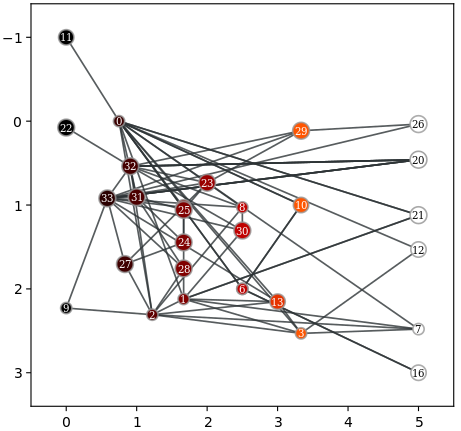
\includegraphics[scale=0.8]{karatelocal.png}
	\caption{Graph generated similarly to the betweenness graph for the karate dataset, but the vertices are plotted with local clustering coefficient as the $x$-axis and trophic levels as the $y$-axis.}
	\label{fig:karatelocal}
\end{figure}

Figure \ref{fig:karatelocal} is shown with local clustering coefficient as the $x$-axis instead. Notice that the clubs with less connections to the major clubs (vertices of high degree) are visually seen to the left in both graphs. These vertices would have a low clustering coefficient as well as a low betweenness. On Figure \ref{fig:karatelocal}, the vertices with the best connections to major clubs are located further to the right of the graph which are the karate clubs 26, 20, 12, etc. However, vertices with high betweenness such as vertex 33 has a smaller local clustering. Due to their club having connections to other smaller clubs, decreasing the overall value of its own connections. This means that clubs on the right have quicker access or communication with larger clubs and are the closest to them.

This concludes the early experimentations on a smaller undirected dataset. We see that the graph properties are successful in identifying correlations and certain vertices that are important. Therefore, instead of using simple datasets, I will generate the datasets based upon different languages as well as their sentence structure. To understand this further, words in languages must be given a rank to judge their importance. This can be demonstrated through \emph{Zipf's Law} discussed in the next section.

\section{Zipf's Law}
Zipf's law analyses the natural languages and the frequency of words that appear in them. Alternatively, Zipf's Law \cite{hosch2009zipf} is generally seen as the frequencies of specific events are inversely proportional to their rank that is determined through this law. The law was proposed by George Kinbgsley Zipf when researching the various frequencies of words within the English language. The law states that the $r^{\text{th}}$ most frequent word in the language has a frequency of $f(r)$ which has a relation with the inverse of $r$. Denoting $r$ as the \emph{frequency rank} for the word and $f(r)$ as the frequency of the word in the corpus examined (The \emph{corpus} means the collection of written text).

\begin{equation}\label{eq:zipfs}
f(r) \propto \frac{1}{r^{\alpha}}
\end{equation}

This is the scale for $\alpha \approx 1$ and means that the most frequent word in the examined text which is $r = 1$ has its frequency of appearance to 1, the next most frequent word which is $r = 2$ has a frequency appearance of $\frac{1}{2^{\alpha}}$ and so on. Zipf's law can be drawn on a graph to show a relation and when $log(f)$ is drawn against $log(r)$, the graph generates a curve that closely resembles a straight line with a slope of $-1$. This is known as Zipf's curve and later in the 1960s, the curve's nature was reinforced by the law being correct for smaller \emph{corpora} (the plural of corpus) \cite{sicilia2002extension}. However, the curve varies depending on the corpora as expected and the higher ranking words deviated more from the straight line. Therefore, Mandelbrot derived a generalisation for Zipf's law to adjust to the frequency distributions within the different languages. Mandelbrot proposed to adjust the rank by a constant $\beta$, demonstrated by

\begin{equation}\label{eq:zipfs}
f(r) \propto \frac{1}{(r + \beta)^{\alpha}}
\end{equation}

Generalisation of Zipf's law can then be applied to various corpora of languages so that a frequency distribution can be viewed for the corpus. An example of this can be seen in Figure \ref{fig:zipfwiki} sourced from \cite{zipffigure}.

\begin{figure}[!htb]
	\centering
	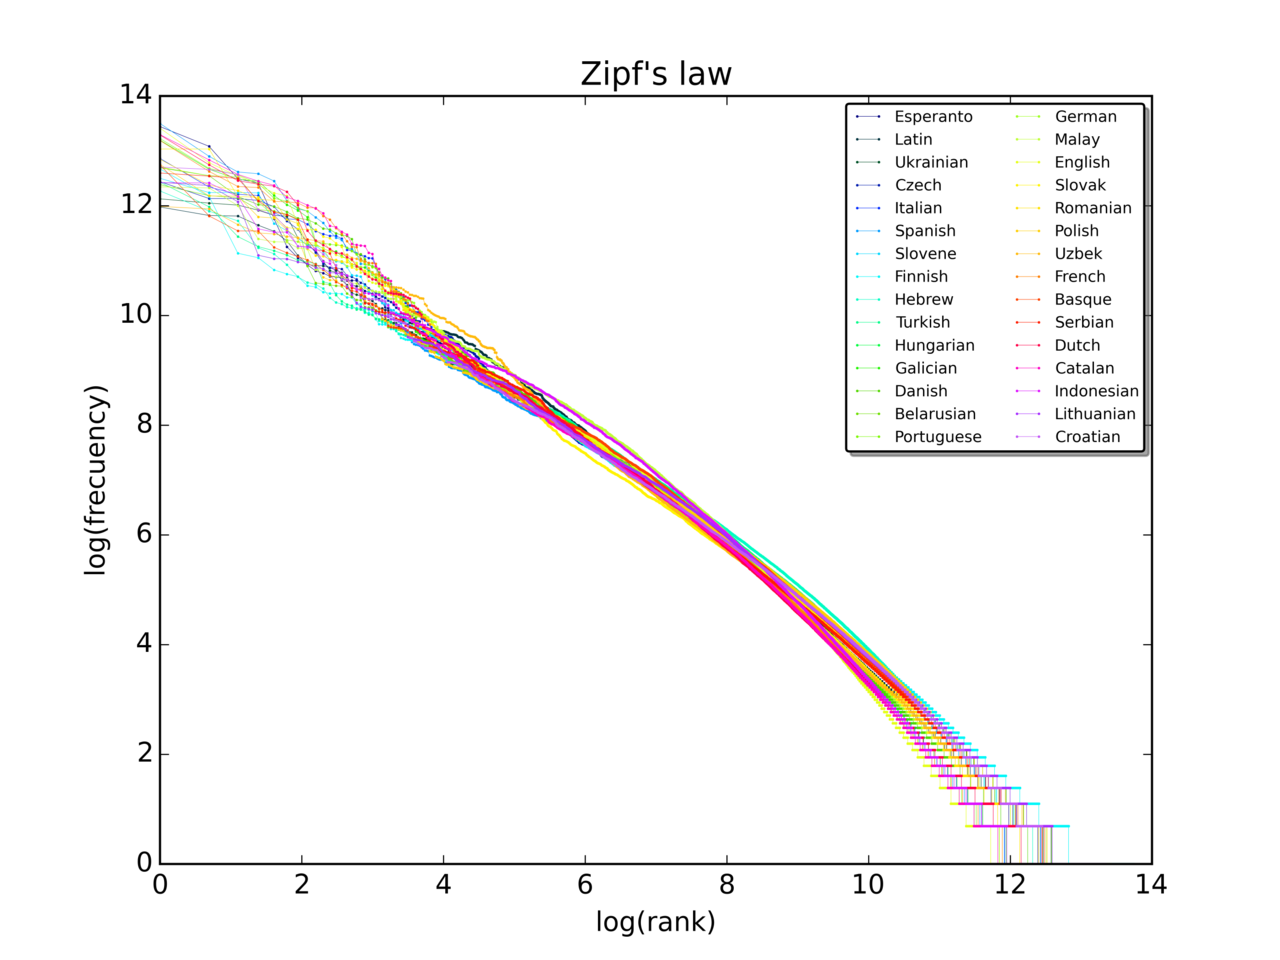
\includegraphics[scale=3]{zipfwiki.png}
	\caption{The plot of Zipf's law containing 30 different language corpora generated from the first 10 million words in each language from Wikipedias.}
	\label{fig:zipfwiki}
\end{figure}

Words in a corpus have a systematic relationship between their rank in their occurrence table. Meaning that they are the words most used such as ``the", ``or", ``of". These words account for most of the word occurrences in the English language. Other words such as ``xylophone" and ``accordion" have the least occurrence in English. A larger corpus is studied by Bentz, Kiela, Hill and Buttery \cite{BentzKielaHillButtery} where they study Zipf's law for Old English and Modern English. They study the frequency and ranks of each word whilst comparing them between the old and new English. In doing so, for old English, the words ``and" is ranked first with a frequency of 1731 whereas in modern English, ``the" is ranked first with a frequency of 1775 and ``and" is second instead with a frequency of 1024. By looking at more words and the comparisons between them, old English has a larger number of distinct words whilst modern English has less. However, modern English has a higher frequency for its first 100 words.

In conclusion, Zipf's Law is a useful tool because languages tend to follow Zipf's curve in terms of their frequencies and rank. Consequently, by following an existing corpus of language, the data can be extrapolated and used in other corpora to determine similarities between the known and the unknown texts. As well as to use it to determine the types of words that are deemed to be most common in a language.